\section{Technischer Hintergrund} \label{sec:technik}
Nachdem ich in den vorherigen Abschnitten versucht habe Ihnen die Konzepte von DMR (Repeater-unabhängige Direkt und Gruppenrufe) näherzubringen, geht es in diesem Abschnitt an das Eingemachte. Da heißt, die technischen Details und Besonderheiten von DMR. Im speziellen um die Begriffe \emph{Time Slot} und \emph{Color Code}.

\subsection{Zeitschlitze (Time Slots)}
Wie zu Beginn erwähnt, ist DMR eine digitale Übertragungstechnik, bei der Sprache zunächst digitalisiert wird, mit einem sogenannten Codec komprimiert wird und als Datenpakete übertragen werden. Modere Sprachcodecs sind in der Zwischenzeit so effizient geworden, dass es möglich ist auf einem $12.5 kHz$ breiten Kanal zwei Sprachsignale in guter Qualität gleichzeitig übertragen zu können. Dies wird auch bei DMR ausgenutzt. DMR verwendet dazu ein Verfahren das sich \adef{TDMA} nennt. 

\begin{figure}[!ht]
 \centering
 \documentclass{standalone}
\newcommand{\repeater}[3]{%
 \node ({#1}) at ({#2}) {%
  \begin{tikzpicture}%
   \draw [black,thick] (-.25,0) -- (0,0.5) -- (0.25,0) -- (-0.25,0);%
   \draw [black,thick,domain=-45:225] plot ({0.2*cos(\x)}, {0.5+0.2*sin(\x)});%
   \draw [black,thick,domain=-45:225] plot ({0.4*cos(\x)}, {0.5+0.4*sin(\x)});%
   \node (xxx) at (0,-.2) {{#3}};%
  \end{tikzpicture}%
 } %
}

\newcommand{\activerepeater}[3]{%
 \node ({#1}) at ({#2}) {%
  \begin{tikzpicture}%
   \draw [black,thick] (-.25,0) -- (0,0.5) -- (0.25,0) -- (-0.25,0);%
   \draw [red,thick,domain=-45:225] plot ({0.2*cos(\x)}, {0.5+0.2*sin(\x)});%
   \draw [red,thick,domain=-45:225] plot ({0.4*cos(\x)}, {0.5+0.4*sin(\x)});%
   \node (xxx) at (0,-.2) {{#3}};%
  \end{tikzpicture}%
 } %
}


\newcommand{\user}[3]{%
 \node ({#1}) at ({#2}) {%
  \begin{tikzpicture}%
   \draw [black,fill=black] (-.25,0) -- (0,0.5) -- (0.25,0) -- (-0.25,0);%
   \draw [black,fill=black] (0,.5) circle (.2); %
   \node (xxx) [text width=0.6cm, align=center] at (-.35cm,-.4) {{#3}};%
  \end{tikzpicture}%
 } %
}

\newcommand{\activeuser}[3]{%
 \node ({#1}) at ({#2}) {%
  \begin{tikzpicture}%
   \draw [red,fill=red] (-.25,0) -- (0,0.5) -- (0.25,0) -- (-0.25,0);%
   \draw [red,fill=red] (0,.5) circle (.2); %
   \node (xxx) [text width=0.6cm, align=center] at (-.35cm,-.4) {{#3}};%
  \end{tikzpicture}%
 } %
}

\begin{document}
 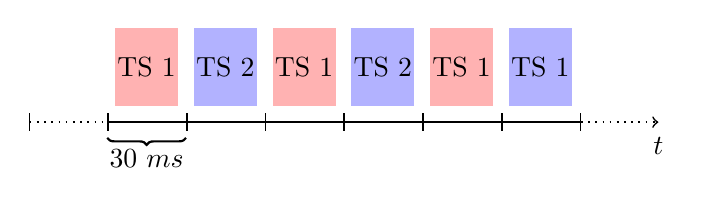
\begin{tikzpicture}
  \draw[|-,dotted, semithick] (-1,-0.2) -- (0,-0.2);
  \draw[|-,semithick] (0,-0.2) -- (1,-0.2);
  \draw[|-,semithick] (1,-0.2) -- (2,-0.2);
  \draw[|-,semithick] (2,-0.2) -- (3,-0.2);
  \draw[|-,semithick] (3,-0.2) -- (4,-0.2);
  \draw[|-,semithick] (4,-0.2) -- (5,-0.2);
  \draw[|-,semithick] (5,-0.2) -- (6,-0.2);
  \draw[|->,dotted,semithick] (6,-0.2) -- (7,-0.2);
  \node at (7, -.5) {$t$};
  \draw [thick,decoration={brace,mirror},decorate] (0,-0.4) -- (1,-0.4) node [pos=0.5, anchor=north,yshift=-0.55] {$30\ ms$}; 
  \fill[red!30] (0.1,0) -- (0.1,1) -- (0.9,1) -- (0.9,0) -- cycle;
  \node at (0.5,0.5) {TS 1};
  \fill[blue!30] (1.1,0) -- (1.1,1) -- (1.9,1) -- (1.9,0) -- cycle;
  \node at (1.5,0.5) {TS 2};
  \fill[red!30] (2.1,0) -- (2.1,1) -- (2.9,1) -- (2.9,0) -- cycle;
  \node at (2.5,0.5) {TS 1};
  \fill[blue!30] (3.1,0) -- (3.1,1) -- (3.9,1) -- (3.9,0) -- cycle;
  \node at (3.5,0.5) {TS 2};
  \fill[red!30] (4.1,0) -- (4.1,1) -- (4.9,1) -- (4.9,0) -- cycle;
  \node at (4.5,0.5) {TS 1};
  \fill[blue!30] (5.1,0) -- (5.1,1) -- (5.9,1) -- (5.9,0) -- cycle;
  \node at (5.5,0.5) {TS 1};  
 \end{tikzpicture}
\end{document}

 \caption{Graphische Darstellung der \emph{time-division multiple access} (TDMA) Technik.}
\end{figure}

Das steht für \emph{time-division multiple access} beschreibt, wie zwei Teilnehmer (quasi) gleichzeitig einen physischen Kanal (also eine Frequenz) benutzen können. Dazu wird jedem der beiden ein Zeitschlitz zu geordnet (Zeitschlitz 1 und 2) und beide senden oder empfangen nur in ihrem eigenen Zeitschlitz. Diese Zeitschlitze sind sehr kurz, bei DMR nur $30ms$ lang. Diese kurze Zeit reicht jedoch aus um $60ms$ lange Sprachfetzen komprimiert zu übertragen. DMR erhält dadurch zwei völlig unabhängige Kanäle pro Frequenz. Das Bedeutet auch, dass zwei völlig unabhängige Gespräche über einen Repeater gleichzeitig laufen können.

Was oder besser wann nun Zeitschlitz 1 oder 2 dran sind, legt der Repeater fest. Er gibt den Takt vor. Das bedeutet auch, dass Zeitschlitze für den Simplexbetrieb völlig unbedeutend sind. Wenn Sie später einen Simplexkanal für Ihr Funkgerät konfigurieren, ist die Zeitschlitzeinstellung egal.

Was auf welchem Zeitschlitz passieren soll, hängt stark von der Konfiguration des einzelnen Repeaters ab. Grundsätzlich gilt aber:
\begin{merke}
 Überregionale Kommunikation sollte auf Zeitschlitz 1 und lokale sowie regionale Kommunikation auf dem Zeitschlitz 2 stattfinden.
\end{merke} 

\subsection{Farbcodes (Color Codes)} \index{Color Code}
Farbcodes sind ein technisches Hilfsmittel, das Störungen zwischen Repeatern vermeiden soll, die auf der selben Frequenz arbeiten. Dieses Problem tritt vor allem im professionellen Einsatz von DMR auf. Einem Unternehmen werden üblicherweise nur wenige Frequenzen zugewiesen, es werden mit unter aber viele Repeater benötigt um ein großes Firmengelände vollständig abdecken zu können (denken Sie an das Flughafenbeispiel). Da bleibt es nicht aus, dass verschiedenen Repeatern die selbe Frequenz zugewiesen werden muss. Wenn sich dann die Reichweiten dieser Repeater überlappen, kann es sein, dass die Aussendungen eines Teilnehmers von zwei Repeatern gleichzeitig aufgenommen werden. Um dies zu verhindern, werden den Repeatern verschiedene sogenannte Farbcodes zugewiesen. Diese kleine zusätzliche Information einer Aussendung erlaubt es einem Repeater oder jedem anderen Teilnehmer zu erkennen, ob eine Aussendung für sie bestimmt ist oder nicht. Nur wenn der Farbcode übereinstimmt, reagiert der Repeater oder das Funkgerät auf diese Aussendung. 

\begin{merke}
 Um einen Repeater nutzen zu können muss nicht nur dessen Ein- und Ausgabefrequenz sondern auch dessen Farbcode bekannt sein!
\end{merke}